\documentclass[a4paper,12pt]{article}   % papír A4, písmo 12 bodu
\usepackage[utf8x]{inputenc}            %kodovaní UTF-8
\usepackage{ucs}                        %kodovani unicode
\usepackage[czech]{babel}               %podpora cestiny
\usepackage[T1]{fontenc}                %pouzij variantu pisma T1 (hacky, carky)
\usepackage[left=2.5cm,right=1.5cm,top=2.5cm,bottom=2.5cm]{geometry} %okraje stranky
\usepackage{amsmath,amsfonts,amssymb}   %podpora matematiky
\usepackage{gensymb,marvosym}           %symboly celsius (\celsius) apod.
%\usepackage{mathptmx}                   %font Times New Roman s~podporou matematiky
\usepackage{times}                      %font Times New Roman (matematika pismem Computer Modern) 
\usepackage{parskip}                    %mezera mezi odstavci
%\usepackage[document]{ragged2e}         %text zarovany vlevo
\usepackage[none]{hyphenat} \sloppy     %slova nedelit a~nepretekat
\usepackage{titlesec}
\setcounter{secnumdepth}{4}
\clubpenalty 10000                      %kontrolovat sirotky
\widowpenalty 10000                     %kontrolovat vdovy
\usepackage{setspace} \onehalfspacing   %podpora pro zmenu radkovani + radkovani 1,5
\usepackage{enumerate}                  %podpora pro zmenu cislovani
\usepackage{fancyhdr}                   %vlastni zahlavi a~zapati
\usepackage{graphicx}                   %podpora grafiky
\graphicspath{{materialy/}}                   %vychozi adresar s~obrazky
\usepackage{caption}                    %popisky
\usepackage{subcaption}                 %podpopisky
\usepackage{siunitx}
\usepackage{MnSymbol,wasysym}
\usepackage[shortlabels]{enumitem}
\usepackage{amsmath}
\usepackage{lastpage}                   %zjištění poslední stránky \pageref{LastPage}
\usepackage{float}                      
\usepackage{url}
\usepackage[unicode]{hyperref}          %klikaci odkazy v~textu
\usepackage{mhchem}
\usepackage{multirow}
\usepackage{tabularx}                   %tabulky se zalamovanim

\usepackage{halloweenmath}


\titleclass{\subsubsubsection}{straight}[\subsection]
\newcounter{subsubsubsection}[subsubsection]
\renewcommand\thesubsubsubsection{\thesubsubsection.\arabic{subsubsubsection}}
\renewcommand\theparagraph{\thesubsubsubsection.\arabic{paragraph}} % optional, useful if paragraphs are to be numbered


%------------------------ čtvrtá a~pátá úroveň nadpisu ---------------------------

\titleformat{\subsubsubsection}
  {\normalfont\normalsize\bfseries}{\thesubsubsubsection}{1em}{}
\titlespacing*{\subsubsubsection}
{0pt}{3.25ex plus 1ex minus .2ex}{1.5ex plus .2ex}

\makeatletter
 
\renewcommand\paragraph{\@startsection{paragraph}{5}{\z@}%
  {3.25ex \@plus1ex \@minus.2ex}%
  {-1em}%
  {\normalfont\normalsize\bfseries}}
\renewcommand\subparagraph{\@startsection{subparagraph}{6}{\parindent}%
  {3.25ex \@plus1ex \@minus .2ex}%
  {-1em}%
  {\normalfont\normalsize\bfseries}}
\def\toclevel@subsubsubsection{4}
\def\toclevel@paragraph{5}
\def\toclevel@paragraph{6}
\def\l@subsubsubsection{\@dottedtocline{4}{7em}{4em}}
\def\l@paragraph{\@dottedtocline{5}{10em}{5em}}
\def\l@subparagraph{\@dottedtocline{6}{14em}{6em}}
\makeatother

\setcounter{secnumdepth}{4}
\setcounter{tocdepth}{4}


\setlist[enumerate]{itemsep=0mm}
%_____________________________|___________________________|_____________________________%
%                             |                           |                             %
%-----------------------------| ZDE VYPLNIT UDAJE O PRACI |-----------------------------%
%_____________________________|___________________________|_____________________________%
%                             

\newcommand{\nazev}{MĚŘENÍ VÝKONŮ A ÚČINÍKU JEDNOFÁZOVÉ ZÁTĚŽE}                                                        %
\newcommand{\jmeno}{Jakub Dvořák}                                                     %
\newcommand{\datum}{27.10.2020}                                                              %
%---------------------------------------------------------------------------------------%


%-----------------------------| POUŽITÁ MAKRA |-----------------------------%

%\newcommand{\zkratka}{ve výsledku se mi napíše tenhle text}
%\newcommand{}{}
%\newcommand{}{}
%\newcommand{}{}
\newcommand{\tsub}[1]{$_\textrm{#1}$}
\newcommand{\texp}[1]{$^\textrm{#1}$}
\newcommand{\tohm}{$\Omega$}


%_______________________________________________________________________________________%
%_______________________________________________________________________________________%


%----------------------------------- KONEC PREAMBULE -----------------------------------%






%-------------------------------------- DOKUMENT --------------------------------------%
%______________________________________________________________________________________%
\begin{document} %%%%%%%%%%%%%%%%%%%%%%%%%%%%%%%%%%%%%%%%%%%%%%%%%%%%%%%%%%%%%%%%%%%%%%%

\setcounter{page}{0} %cislo strany
\pagestyle{empty} %stranku necislovat

%prostredi pro grafy a~schemata \begin{graf} \begin{schema}
\newfloat{schema}{htbp}{schema}\floatname{schema}{Schéma}
\newfloat{graf}{htbp}{graf}\floatname{graf}{Graf}

\begin{titlepage}
    \begin{center}
        \vspace*{1cm}
            
        \Huge
        \textbf{\nazev}
            
        \vspace{0.5cm}
        \LARGE
            
        \vspace{1.5cm}
            
        \textbf{\jmeno}
            
        \vfill
            
        \vspace{0.8cm}
            
        \Large
            
        \datum\\
        \vspace*{.5cm}
        
\includegraphics[width=.4\textwidth]{logo-cvut-fee.png}\\
    \end{center}
\end{titlepage}

% --- definice zapati a~cislovani ---
\newpage 
\pagestyle{fancy}                                       %vlastni zahlavi/zapati
\renewcommand{\headrulewidth}{0pt}                      %bez linky v~zahlavi
\renewcommand{\footrulewidth}{.5pt}                    %linka v~zapati - optional
\lhead{}       \chead{} \rhead{\nazev}                        %pole zahlavi (prazdna)
\lfoot{\jmeno} \cfoot{} \rfoot{\thepage}   %pole zapati


%------------------------------------ VLASTNÍ TEXT ------------------------------------%



\section{Úkol měření}
\label{chap:zadani}
\begin{enumerate}
  \item  Změřte činný výkon, účiník a~zdánlivý výkon jednofázové zátěže. K měření použijte univerzální klešťový přístroj s číslicovým zobrazením, činný výkon změřte rovněž pomocí ručkového wattmetru a~měřicího transformátoru proudu (MTP). Při měření činného výkonu určete v~obou případech rozšířenou nejistotu typu B ($k_r$~=~2). U výsledků měření pomocí ručkového wattmetru korigujte chybu metody, chybu úhlu MTP zanedbejte. Posuďte, zda rozdíl hodnot měřených oběma přístroji odpovídá jejich uvedené přesnosti.
  \item  Změřte napětí na sekundárním vinutí MTP a~zkontrolujte, není-li překročeno dovolené zatížení transformátoru.
\end{enumerate}



\section{Schéma zapojení}
\label{schema_zapojeni}
\begin{figure}[h!]
  \centering
  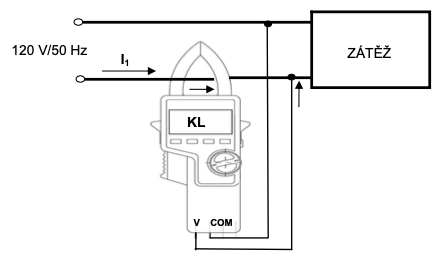
\includegraphics[width=.6\textwidth]{kestewatt.png}
  \caption{Měření činného výkonu, účiníku a~zdánlivého výkonu pomocí univerzálního klešťového přístroje}
  \label{fig:klestewatt}
\end{figure}

\begin{figure}[h!]
  \centering
  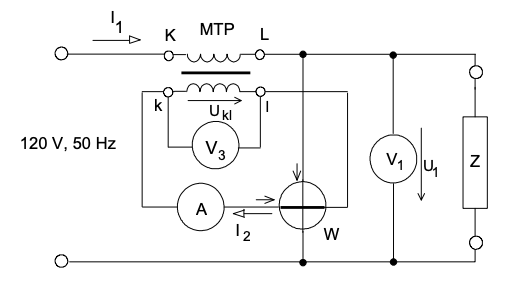
\includegraphics[width=.6\textwidth]{rucwatt.png}
  \caption{Zapojení pro měření činného výkonu jednofázové zátěže pomocí ručkového wattmetru}
  \label{fig:rucwatt}
\end{figure}

\section{Seznam použitých přístrojů}
\begin{table}[h!]
  \begin{tabularx}{\textwidth}{lX}
    KL &    - univerzální klešťový přístroj s číslicovým zobrazením PK 430.1\\
    A  &    - ampérmetr elektromagnetický, tř.přes. 0,5, použitý rozsah 10~A\\
    V\tsub{1}  &- voltmetr magnetoelektrický s usměrňovačem, tř.přes. 1,5, použitý rozsah 240, odpor 5000~\tohm , tj. 1,2~M~\tohm \\
    W &     - wattmetr elektrodynamický, tř.přes. 0,5, napěťový rozsah 240~V, proudový rozsah 2~A, odpor napěťové cívky 8~k\tohm  \\
    MTP &   - měřicí transformátor proudu, převod 1:3 chyba fáze 30~úhl.~minut, chyba převodu není známa \\
    120~V&  - zdroj střídavého napětí - rozvaděč\\
    Z &     - měřená zátěž\\
  \end{tabularx}
\end{table}


\section{Teoretický úvod}
\label{chap:uvod}
Při měření analogovým wattmetrem je potřeba dbát na rozsah jak napěťový, tak proudový. Jelikož proud, který bychom měřili, by byl mimo rozsah wattmetru, použili jsme měřicí transformátor proudu, kterým jsme 3$\times$ snížili měřený proud. Tím jsme bohužel zavedli novou nejistotu, se kterou musíme počítat. Zároveň při použití transformátoru nesmí být překročena hodnota zdánlivého výkonu $S_j$, po které již přestává platit daná chyba převodu a~chyba fáze. Hodnota $S_j$ je dána vztahem:
\begin{equation*}
  S_j~=~U_{klj}I_{2j}~=~Z_{2j}I^2_j~~\textrm{[VA]},
\end{equation*}
kde 
\begin{tabularx}{\textwidth}{ll}
  $I_{2j}$ & je jmenovitá hodnota sekundárního proudu MTP (zpravidla 5 A),\\
  $U_{klj}$ & je úbytek napětí na svorkách k-l MTP (viz obr. \ref{fig:rucwatt}) odpovídající proudu $I_{2j}$ a~jmenovité impedanci $Z_{2j}$ zapojené v~sekundáru MTP.
\end{tabularx}

Velikost měřeného činného výkonu pomocí analogového wattmetru zjistíme podle odečtu dílků, které ukazuje ručička. Jeden dílek je roven hodnotě $k_W$, která lze spočítat jako
\begin{equation*}
  k_W~=~\frac{rozsah_U \cdot rozsah_I}{rozsah_{stupnice}}
\end{equation*}

Při měření veličin klešťovým přístrojem vypočítáme nejistotu resp. rozšířenou nejistotu podle vztahu
\begin{equation*}
  U_P~=~k_r\cdot \frac{\delta_{P_R}\cdot R_{P_R}}{100\sqrt{2}}~~\textrm{[W]}.
\end{equation*}

Velikost měřeného činného výkonu $P_m$ určíme ze vztahu
\begin{equation*}
  P_m~=~U_1 I_1 cos\,\varphi~=~P_W \cdot p_I,
\end{equation*}
kde $P_W$ je údaj wattmetru.

Hodnota $P_m$ je zatížena chybou metody, která přestavuje vlastní spotřebu pro pohyb ručičky. Tuto chybu lze korigovat pomocí vztahu \ref{eq:korig}, čímž dostaneme korigovanou hodnotu výkonu $P_K$
\begin{equation}
  P_K~=~P_m - \frac{U_1^2}{R_{nW}R_V}(R_{nW} + R_V)
  \label{eq:korig}
\end{equation}

Skutečná hodnotu činného výkonu, kterou zátěž odebírá je dána vztahem $P_m~=~P_W p_I$. Nejistota měření výkonu odebíraného zátěží se potom určí ze vztahu
\begin{equation}
  u_{P_m}~=~\sqrt{\left(\frac{\partial P_m}{\partial P_W}u_{P_W}\right)^2 + \left(\frac{\partial P_m}{\partial p_I}u_{p_I}\right)}~=~\sqrt{(p_I \cdot u_{P_W})^2 + (P_W \cdot u_{p_I})^2},
  \label{eq:analognejistota}
\end{equation}
kde
\begin{equation}
  u_{P_W}~=~\frac{TP_W\cdot M_W}{100\sqrt{3}};~u_{p_I}=\frac{TP_{MTP} \cdot p_I}{100\sqrt{3}}. 
\end{equation}


Nejistotu digitálního wattmetru spočítáme standardním vzorcem 
\begin{equation}
  u(W_D)~=~\frac{\delta_R\cdot R_U R_I}{100\cdot\sqrt{3}}
  \label{eq:diginejistota}
\end{equation}


\section{Naměřené hodnoty}
Naměřené hodnoty jsou v~tabulce \ref{tab:nam}
\begin{table}
  \centering
  \begin{tabular}{|c|c|c|c|c|c|c|}
    \hline
    &$\textrm{V}_\textrm{1}$[V]&$\textrm{A}_\textrm{1} $[A]&$\textrm{W}_\textrm{A} $[dílky]&$\textrm{U}_\textrm{3}$[V]&$\textrm{W}_\textrm{D}$ [W]&$\textrm{W}_\textrm{D}$ cos\,$\varphi$[1]\\\hline\hline
    Měřená hodnota&126&4,6&74&2,5&2781&0,51\\\hline
    Přepočtená hodnota&&13,8&296~W&&927&\\\hline
  \end{tabular}
  \caption{Naměřené hodnoty}
  \label{tab:nam}
\end{table}




\section{Zpracování naměřených hodnot}

\begin{table}[h!]
  \centering
  \begin{tabular}{|l|l|}
    \hline
    Zdánlivý výkon z napětí a~proudu &1738,8~VA\\\hline
    Činný výkon z napětí a~proudu &886,79~W\\\hline
    Analogový wattmetr &888~W\\\hline
    Digitální wattmetr &927~W\\\hline
  \end{tabular}
  \caption{Přepočtené hodnoty}
  \label{tab:spocteno}
\end{table}
\subsection{Nejistota digitálních wattmetru}
Nejistotu měření digitálním přístrojem, popsanou v~kapitole \ref{chap:uvod}, spočítáme pomocí vzorce \ref{eq:diginejistota}.
\begin{equation*}
  u(W_D)~=~2\cdot\frac{\delta_R\cdot R}{100\cdot\sqrt{3}}~=~2\cdot \frac{\frac{2}{100}\cdot 3999}{\sqrt{3}}~W~=~92,35~W.
\end{equation*}
\section{Nejistota analogového wattmetru}
Pro rozšířenou nejistotu měření analogovým přístrojem budeme vycházet z rovnice \ref{eq:analognejistota}, kde po dosazení dílčích nejistot dostaneme
\begin{equation*}
  \sqrt{\left(p_I \cdot \frac{TP_W\cdot M_W}{100\sqrt{3}}\right)^2 + \left(P_W \cdot \frac{TP_{MTP} \cdot p_I}{100\sqrt{3}}\right)^2}
\end{equation*}
a po dosazení hodnot dostaneme
\begin{equation*}
  2\cdot\sqrt{\left(3 \cdot \frac{0,5\cdot 2400}{100\sqrt{3}}\right)^2 + \left(888 \cdot \frac{0,5 \cdot 3}{100\sqrt{3}}\right)^2}~=~6,6~W
\end{equation*}
\section{Korekce chyby měření analogovým wattmetrem}
\begin{equation*}
  R_{n_W}~=~8000~\Omega; R_V~=~1,2~M\Omega; U_1~=~126~V; P_m~=~888~W.
\end{equation*}
\begin{equation*}
  P_K~=~P_m - \frac{U_1^2}{R_{nW}R_V}(R_{nW} + R_V)~=~888 - \frac{126^2}{8000\cdot 1\,800\,000}\cdot (8000 + 1\,800\,000)~=~886~W
\end{equation*}

\section{Závěrečné vyhodnocení}
Činný výkon naměřený digitálním měřákem je $P_D$927\,$\pm$\,92,35~W. Účiník jsme naměřili $cos\,\varphi$~=~0,51. Korigovaná hodnota wýkonu měřeného analogovým wattmetrem vyšla~W$_\textrm{K}$~=~886~W. Hodnota nekorigovaná vyšla 888\,$\pm$\,6,6~W.

%--- LITERATURA a~ZDROJE (povinne) ---
\clearpage
\renewcommand{\refname}{Seznam použité literatury a~zdrojů informací} 
%\section*{Seznam použité literatury a~zdrojů informací}
\phantomsection %pridej odkaz do PDF zalozek
\addcontentsline{toc}{section}{Seznam použité literatury a~zdrojů informací}

\begin{thebibliography}{99}

%----------------------------------------------------
\subsection*{Seznam použitých internetových zdrojů}
    \bibitem{navod} Návod k~laboratorní úloze
    
\end{thebibliography}

\end{document}